% !TeX root = ../libro.tex
% !TeX encoding = utf8

\chapter{Conceptos previos}

Este capítulo tiene el objetivo de introduccir los conceptos básicos utilizados en esta primera parte del proyecto. Dichos conceptos se han obtenido de las referencias \cite{MorseTh1}, \cite{MorseTh2} y \cite{Triangulacion}, junto con el conocimiento adquirido de las asignaturas de Topología II y Variedades Diferenciables.

\begin{definicion} Una \textbf{variedad topológica} 2-dimensional es un espacio de Hausdorff localmente Euclídeo que verifica el segundo axioma de numerabilidad, es decir, su topología tiene una base numerable.
\end{definicion}

\begin{definicion} Un \textbf{embebimiento o encaje} es una aplicación continua e inyectiva de un espacio topológico en otro. La restricción de su imagen aporta un homeomorfismo.
\end{definicion}

\begin{definicion} Un \textbf{sistema coordenado} sobre $S$ es un embebimiento $h : \mathbb{R}^2 \rightarrow S$.
\end{definicion}

\begin{definicion} Sea $S$ un espacio topoógico Hausdorff, un \textbf{atlas} $2-dimensional$ sobre $S$ es una familia de cartas $E=\{h_i\}_{i\in \Lambda}$ verificando:
	\begin{enumerate}
		\item $\{h_i(\mathbb{R}^2)\}_{i\in \Lambda}$ es un recubrimiento abierto de $S$.
		\item Si $h_i(\mathbb{R}^2) \cap h_j(\mathbb{R}^2) \neq \varnothing$ entonces $h_j^{-1} \circ h_i:h_i^{-1}(h_i(\mathbb{R}^2)\cap h_j(\mathbb{R}^2)) \rightarrow h_j^{-1}(h_i(\mathbb{R}^2)\cap h_j(\mathbb{R}^2))$ es un difeomorfismo.
	\end{enumerate}
\end{definicion}

\begin{definicion} Sea $S$ un espacio topoógico Hausdorff, una \textbf{estructura diferenciable} $2-dimensional$ sobre $S$ es un atlas maximal.
\end{definicion}

\begin{definicion} Una \textbf{variedad diferenciable} 2-dimensional es una variedad topológica $2-dimensional$ $S$ junto con una estructura diferenciable $E$, es decir, el par $(S, E)$.
\end{definicion}

\begin{definicion} Una \textbf{inmersión} es una aplicación diferenciable entre variedades diferenciables cuya derivada es inyectiva en todo punto.
\end{definicion}

\begin{definicion} Una \textbf{celda} $C$ es un subconjunto abierto de un espacio topológico $X$ tal que $C$ homeomorfa a la bola unidad n-dimensional, que se puede extender de forma continua al borde. Dicho homeomorfismo se denomina $\textbf{aplicación celda}$. Si esta aplicación es diferenciable, se dice que la celda es diferenciable.
\end{definicion}

\begin{definicion} Una \textbf{triangulación diferenciable} de una variedad $X$ es un conjunto de celdas diferenciables tal que la unión de todas ellas es $X$ y cuyas intersecciones son únicamente los lados, es decir, los interiores son disjuntos $2$ a $2$.
\end{definicion}
\newpage
\begin{definicion} Sean $f$ y $g$ homeomorfismos entre los espacios topológicos $X$ e $Y$. Una \textbf{isotopía} es una homotopía entre $f$ y $g$, $H: X \times [0,1] \rightarrow Y$, con:
	\begin{enumerate}
		\item $H_0 = f$.
		\item $H_1 = g$.
		\item $\forall t \in [0,1]$, $H_t$ es un homeomorfismo.
	\end{enumerate}
\end{definicion}

\begin{definicion} Sean $f$ y $g$ embebimientos entre las variedades $N$ e $M$. Una \textbf{isotopía de embebimientos} es un homeomorfismo $H: M \times [0,1] \rightarrow M \times [0,1]$ cumpliendo:
	\begin{enumerate}
		\item $H(y, 0) = (y, 0)$ $\forall y \in M$.
		\item $H(f(x), 1) = (g(x), 1)$ $\forall x \in N$.
		\item $H(M \times \{t\}) = M \times \{t\}$ $\forall t \in [0,1]$.
	\end{enumerate}
	
	Equivalentemente podemos decir que $H$ es la isotopía de $Id_M$ en $g \circ f^{-1}$ donde tenga sentido.
\end{definicion}

\begin{definicion} Sea $M$ una variedad diferenciable y $f: M \rightarrow \R$ una función diferenciable en $M$. Un punto $p \in M$ se dice que es un $\textbf{punto crítico}$ de $f$ si $Df(p) = 0$ en $T_pM$. A su imagen por $f$, $f(p)$, se le dice $\textbf{valor crítico}$ de $f$.
\end{definicion}

\begin{definicion} Sea $M$ una variedad diferenciable y $f: M \rightarrow \R$ una función diferenciable en $M$. Un punto crítico $p \in M$ se dice que es $\textbf{no degenerado}$ si $H_\phi(f)(p)$ es regular para cualquier parametrización $\phi$ centrada en $p$, donde $H_\phi(f)=H(f \circ \phi)$ la matriz Hessiana de $f \circ \phi$.\\ 
\\ El $\textbf{índice}$ de dicho punto es la dimensión del mayor subespacio de $T_pM$ donde $H_\phi(f)$ es definida negativa. No depende de $\phi$ por la regla de Sylvester, ya que $H$ para otra parametrización $\psi$ cumple $H_\psi(f) = J^t(\theta) H_\phi(f) J(\theta)$, con $\theta$ el cambio de coordenadas y $J$ la matriz Jacobiana.
\end{definicion}

\begin{definicion} Sea $f$ una función diferencaible en una superficie $S$, se dice que es una $\textbf{función de Morse}$ si todos sus puntos críticos son no degenerados.
\end{definicion}

\newpage
\begin{definicion} Sea $f$ una función de Morse, dados $a < b$ valores regulares de $f$ en $\R$ definimos:
	\begin{itemize}
		\item $V(a) = f^{-1}(a)$, se puede ver como una curva de nivel.
		\item $M(a) = f^{-1}((-\infty, a])$, el conjunto que hay ``debajo'' de la curva de nivel cuyo valor es $a$.
		\item $M'(a) = f^{-1}([a,\infty))$, el conjunto que hay ``encima'' de la curva de nivel cuyo valor es $a$.
		\item $W(a,b) = f^{-1}([a,b])$, el conjunto contenido entre 2 curvas de nivel.
	\end{itemize}
\end{definicion}

\begin{figure}[h]
  	\centering
  	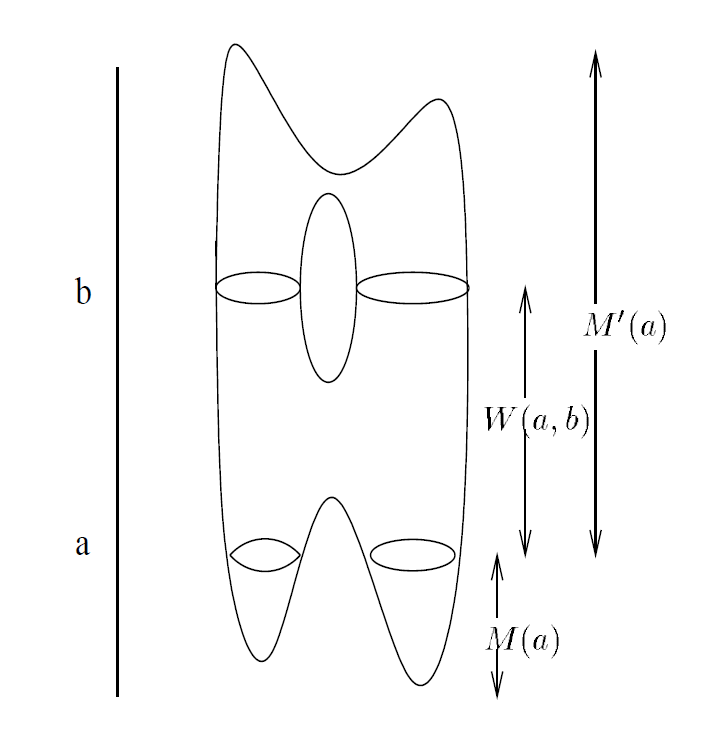
\includegraphics[width=0.4\textwidth]{niveles_morse}
  	\label{fig:niveles_morse}
\end{figure}

\endinput
%------------------------------------------------------------------------------------
% FIN DEL CAPÍTULO. 
%------------------------------------------------------------------------------------
